\documentclass[usenatbib]{aastex}
\usepackage{amsmath,amssymb}
%\usepackage{natbib}
\usepackage{graphicx} 
\begin{document}

\section{Science Justification}
Weak gravitational lensing has been widely touted as a powerful probe of cosmology. It is a major science driver for several large imaging surveys, such as the Dark Energy Survey (DES) the Large Synoptic Survey Telescope (LSST), and space missions such as Euclid and the Wide-Field Infrared Survey Telescope (WFIRST). Weak lensing is weak, however, and all current measurements are limited by the scatter in galaxy shapes, which is an order of magnitude or more greater than the typical weak lensing signal. This means that weak lensing analyses must average over every available galaxy image, pushing the analysis to include faint and poorly-resolved galaxies for which unbiased measurements of galaxy shapes are difficult. Precision estimates of galaxy redshifts from photometry is crucial for these analyses, as the current generation of ongoing surveys will entail sample sizes of a few $\times10^8$ galaxies, which is two orders of magnitude beyond the size of the largest existing spectroscopic samples. Percent-level biases in the photometric redshifts will have a large impact on the error budgets for this next generation of surveys.

Here we propose a pilot study for a new weak lensing measurement technique that uses the Tully-Fisher relation (TFR) to obviate the photo-z and shear calibration problems while offering a very large reduction in the effective lensing noise.

Disk galaxies are inclined at random with respect to the line of sight to the observer, so the measured rotation velocity is related to the true circular velocity of the disk by $v_{\rm obs} = v_{\rm circ} \sin i$. Correcting for the effects of inclination has been an important obsevational complication inherent in TFR studies to date. Typically observers model the galaxy as a thin disk and estimate $\sin i$ from the ellipticity of the image.

After inclination correction, estimates for the intrinsic fractional scatter in $v_{\rm circ}$ at fixed luminosity or stellar mass are typically .05 dex or less. If the TFR is regarded as known, then a galaxy's velocity offset from the relation becomes a estimator for its true unlensed ellipticity. Properly weighted, the scatter in the ellipticity estimated this way is only .015 -- in other words, knowledge of the disk inclination controls for 95\% of the variation in the observed shape of the disk. This quantity is sensitive to measurement errors in $v_{\rm circ}$, as shown in figure~\ref{fig:shapeNoise}; in general, rotation curve errors of $10 $ km/s reduce the disk galaxy shape noise by an order of magnitude.



\begin{figure}[t]
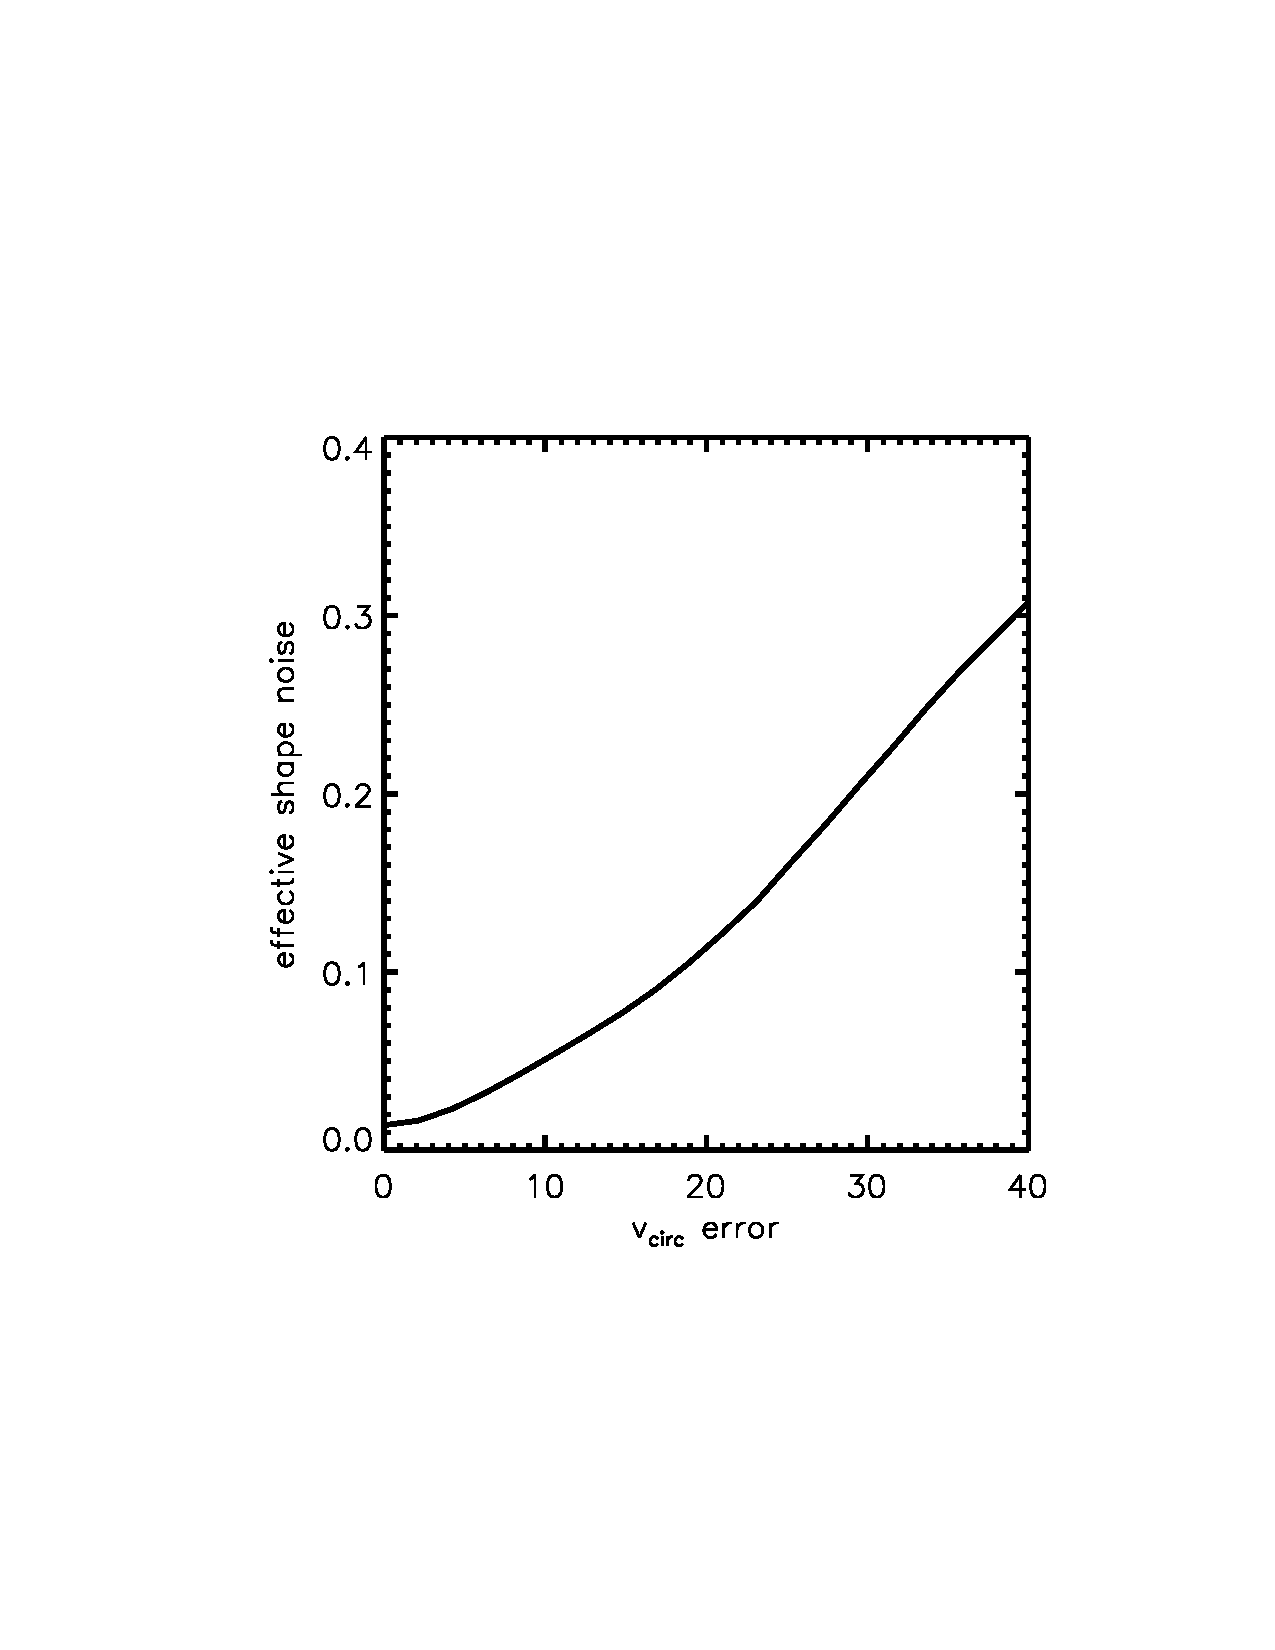
\includegraphics[width=\linewidth, bb= 150 150 550 650,clip]{Plots/vcirc_error.pdf}
\caption{Effective shape noise $\sigma_{TF}$ as a  function of the
  measurement error on the disk circular velocity.}
\label{fig:shapeNoise}
\end{figure}

\subsection{}


\subsection{A Pilot Study for a Stage V Dark Energy Experiment}

\end{document}